\documentclass{article}

%other packages
\usepackage[a4paper]{geometry}
\usepackage{longtable}
\usepackage{wrapfig}
\setlength\parindent{0pt}
\usepackage{enumitem}
\usepackage[table,dvipsnames]{xcolor}
\usepackage{polynom}
\def\scaleint#1{\vcenter{\hbox{\scaleto[3ex]{\displaystyle\int}{#1}}}}
\usepackage{array}
\newcolumntype{C}{>{{}}c<{{}}} % for '+' and '-' symbols
\newcolumntype{R}{>{\displaystyle}r} % automatic display-style math mode 
\usepackage{tabularray}
\usepackage{dcolumn,tabularx,booktabs}
\usepackage[most]{tcolorbox}

%maths
\usepackage{mathtools}
\usepackage{amsmath}
\usepackage{amssymb}
\usepackage{amsfonts}
\usepackage{autobreak}

%tikzpicture
\usepackage{tikz}
\usepackage{scalerel}
\usepackage{pict2e}
\usepackage{tkz-euclide}
\usepackage{tikz-3dplot}
\usetikzlibrary{calc}
\usetikzlibrary{patterns,arrows.meta}
\usetikzlibrary{shadows}
\usetikzlibrary{external}
\usetikzlibrary{decorations.pathreplacing,angles,quotes}

%pgfplots
\usepackage{pgfplots}
\pgfplotsset{compat=1.18}
\usepgfplotslibrary{statistics}
\usepgfplotslibrary{fillbetween}

\pgfplotsset{
    standard/.style={
    axis line style = thick,
    trig format=deg,
    enlargelimits,
    axis x line=middle,
    axis y line=middle,
    enlarge x limits=0.15,
    enlarge y limits=0.15,
    every axis x label/.style={at={(current axis.right of origin)},anchor=north west},
    every axis y label/.style={at={(current axis.above origin)},anchor=south east}
    }
}

\begin{document}

\begin{center}
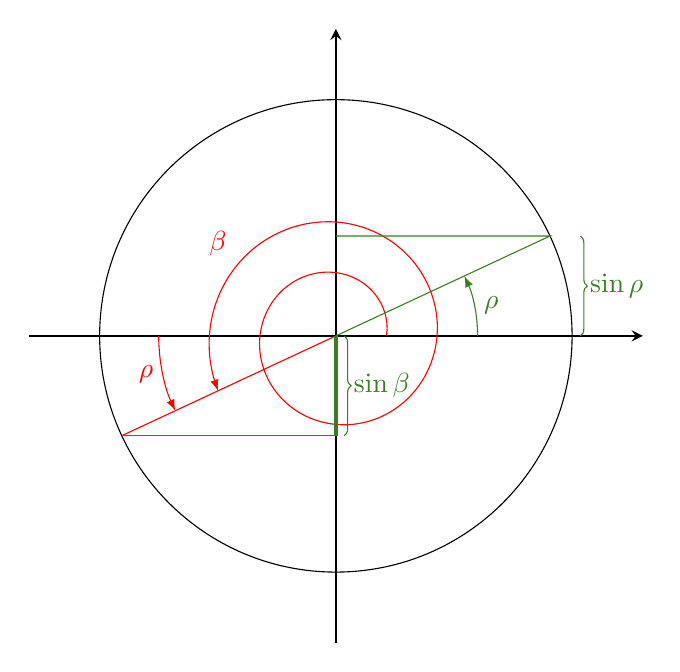
\begin{tikzpicture}[scale=3]
\draw[thick,-stealth] (0,-1.3) -- (0,1.3);
\draw[thick,-stealth] (-1.3,0) -- (1.3,0);
\coordinate (O) at (0,0);
\draw[] (O) circle [radius=1];
\draw[-latex,domain=360:925,variable=\t,smooth,samples=75,red] plot ({\t}: {0.0006*\t});
\node[above left] at (865:0.0006*865) {${\color{red}\beta}$};
\draw[red] (O) -- (925:1);
\draw[red,-latex] (-0.75,0) arc [start angle=180, end angle=205, radius=0.75] node[pos=0.5,left]{$\rho$};
\draw[OliveGreen] (O) -- (25:1) -- (0,0.42262);
\draw[OliveGreen] (925:1) -- (0,-0.42262);
\draw[OliveGreen,very thick] (O) -- (0,-0.42262);
\draw[OliveGreen,-latex] (0.6,0) arc[start angle=0, end angle=25, radius=0.6] node[pos=0.5,right]{$\rho$};
\draw [decorate,color=OliveGreen, decoration = {brace,mirror,raise=3pt}] (0,-0.42262) -- (O) node[pos=0.5,right=3pt,OliveGreen]{$\sin\beta$};
\draw [decorate,color=OliveGreen, decoration = {brace,mirror,raise=3pt}] (1,0) -- (1,0.42262) node[pos=0.5,right=3pt,OliveGreen]{$\sin\rho$};
\end{tikzpicture}
\end{center}

\end{document}